\section{Introdução}

Este projeto tem como objetivo a criação de um \textit{device driver} para a
plataforma Linux e um vírus específico para este \textit{driver}, além de 
realizar estudo sobre os dois temas.

\subsection{\textit{Device Driver}}

Um \textit{device driver} é um mecanismo especial do Linux kernel que permite
ao programador construir uma lógica através de uma interface de comunicação
com um dispositivo de IO (\textit{Input and Output}). Com essa interface
o \textit{driver} pode ser construído a parte do resto do kernel e "plugado" em tempo
real quando necessário.

Na construção de um \textit{device driver}, é importante esclarecer dois conceitos:
\begin{itemize}
  \item \textit{\textbf{Kernel Space}}: o kernel gerencia o \textit{hardware} de maneira simples, oferecendo
    ao usuário um simples e uniforme modo de programação, as interfaces. Sendo assim,
    o kernel promove uma ponte entre o usuário/programador e o \textit{hardware}. Qualquer
    subrotina e função que façam parte do kernel são considerados parte do \textit{kernel space}.

  \item \textit{\textbf{User Space}}: os programas \textit{end-user} como o UNIX shell ou outra aplicação GUI são
    parte do \textit{user space}. Elas se comunicam com o \textit{hardware} do sistema, mas não diretamente.
    O kernel promove funções de suporte para essas aplicações e o próprio kernel realiza
    a gerência do \textit{hardware}.

\end{itemize}

\begin{figure}[H]
  \centering
  \caption{\textit{User Space} onde as aplicações residem, e \textit{Kernel Space} onde modulos e \textit{device drivers} residem }
  \label{fig:usblinux}
  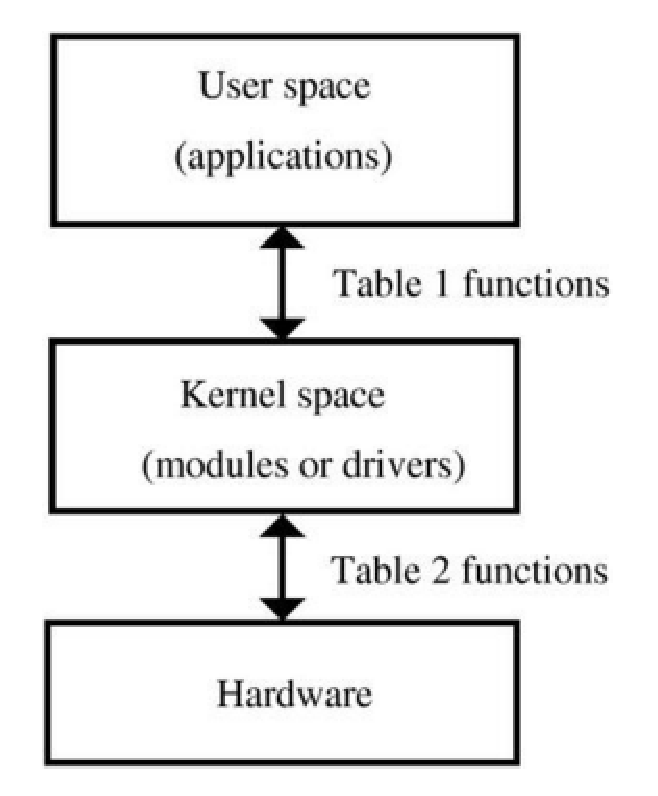
\includegraphics[width=0.3\textwidth]{figure/kernel.eps}
\end{figure}

Em resumo, kernel oferece subrotinas ou funções para as aplicações \textit{end-user} para interagir
com o \textit{hardware} (user space), mas também oferece funções para a comunicação baixo nível do sistema
com o \textit{hardware} (kernel space).

\subsubsection{USB Driver}

Em um sistema operacional Linux, um dispositivo USB sempre será detectado quando inserido.
A detecção em nível de \textit{hardware} é feito pela controladora de USB - \textit{USB Host Controller}. A controladora
correspondênte irá enviar as informações da camada \textit{low-level} para a camada \textit{higher-level} que contém
as especificações do protocolo USB. As especificações de protocolo transformam as infomações recebidas
sobre o dispositivo e os propaga para a camada de USB genérica - \textit{USB Core} - definida no espaço
do kernel. Nesse ponto, o device é detectado mesmo sem haver um \textit{driver} associado específicamente a ele.

\begin{figure}[H]
  \centering
  \caption{Camadas do sistema USB Linux}
  \label{fig:usblinux}
  \includegraphics[width=0.9\textwidth]{figure/usbgeral.eps}
\end{figure}

A camada de USB core se comunica com o dispositivo utilizando os \textit{urb} que é descrito com uma estrutura
(\textit{struct urb}). Os urbs são utilizado para enviar e receber dados de um USB endpoint de um
dispositivo específico. O ciclo de vida de um urb é basicamente:
\begin{enumerate}
  \item Criado por um driver;
  \item Associado a um endpoint de um dispositivo USB;
  \item Submetido para o USB code pelo driver;
  \item Submetido para o USB host controller específico do dispositivo;
  \item Processado pelo USB host controller que transfere para o dispositivo;
  \item Quando o urb é completado, o USB host controller notifica o driver.
\end{enumerate}

Um urb é criado dinamicamente e  pode ser concelado a qualquer momento pelo driver ou pelo USB core
se o dispositivo for removido do sistema.

Um dispositívo válido de USB tem uma estrutura composta por: \textit{configurations, interface e endpoints}.
\begin{itemize}
  \item \textbf{Configurations}: é o perfil do dispositivo. É usado pelo USB Core para inicializar o dispositivo;
  \item \textbf{Interface}: corresponde a funcionalidade do dispositívo;
  \item \textbf{Endpoint}: são como \textit{pipes} que transferem informações para o dispositívo ou para o computador.
\end{itemize}

O ambiente Linux suporta apenas uma \textit{configuration} por dispositivo. Para cada \textit{configuration}, o dispositivo
pode tem uma ou mais \textit{interface}. Como dito, uma \textit{interface} representa uma funcionalidade do dispositivo,
por exemplo, uma impressora multifuncional tem as funções de imprimir, scanner e fax. Portanto, um
dispositivo USB, ao contrário de outros dispositivos, é associado por \textit{interface} ao invés do dispositivo
como um todo. Em resumo, um dispositivo USB pode tem vários drivers e várias \textit{interfaces} podem ter o
mesmo driver. E para cada \textit{interface} tem-se vários \textit{endpoints}. A figura \ref{fig:usbdevice} mostra essa
estrutura.

\begin{figure}[H]
  \centering
  \caption{Estrutura de um dispositivo.}
  \label{fig:usbdevice}
  \includegraphics[width=0.9\textwidth]{figure/usbdevice.eps}
\end{figure}

Na seção \ref{utils} será mostrado algumas aplicações e comandos que são utilizados para identificar
as informações de um dispositivo USB.


\subsection{Vírus}

\section{Descrição do Problema}

Dentro do contexto de \textit{device drivers}, existe o aspecto de segurança do sistema operacional.
Ataques externos são considerados qualquer tentativa de recuperar dados sigilosos, danificar
o sistema em sí ou utilizar recursos computacionais para realizar outras operações não autorizadas.
Com visão deste cenário, será necessário construír um vírus para um \textit{driver} específico.
No caso deste projeto, o vírus será direcionado para um \textit{driver} construído especificamente para
este objetivo, contendo dois comportamentos: normal e anormal, para apresentar o
funcionamento do vírus.

\section{Metodologia}

O grupo adotou reuniões presenciais e remotas para desenvolvimento do trabalho. A partir
disso algumas ferramentas foram utilizadas para que se pudesse desenvolver o trabalho em
equipe. As ferramentas foram:

\begin{itemize}
  \item Google hangout;
  \item Tmate;
  \item Github;
\end{itemize}

O Google hangout fora utilizado em conjunto com o tmate para provimento de reuniões remotas
e compartilhamento do terminal respectivamente. O tmate com seu compartilhamento de terminal
via ssh permite todos integrantes tenham acesso á um terminal único em tempo real. Desse modo,
o pareamento remoto torna-se facilitado. O Github é utilizado como ferramento de versionamento
de código. 

\section{\textit{Checklist} de Requisitos}

A lista abaixo contem os requisitos espeficicados para o laboratório e o
seu status de implementação da solução proposta.

\begin{itemize}
  \item (OK ) Estudo sobre Vírus: tipos de vírus e vermes, como eles se disseminam;
  \item (OK) Estudo sobre \textit{Device Drivers}: funcionamento e como construir;
  \item (OK) Tutorial da construção do \textit{Device Drivers} (Anexo A);
  \item (  ) Propor um \textit{Device Drive} com duas forma de funcionamento: normal e anormal;
  \item (OK) O \textit{Device Drive} deve ser gerenciado por lsmdo, insmod, rmmod;
  \item (OK) O \textit{Device Drive} deve apresentar na tela o que está ocorrendo;
  \item (OK) Usar processos em ambiente Linux/Linguagem C;
  \item (  ) Executar o programa várias vezes e criar um quadro adequado para apresetar os resultados;
\end{itemize}

\section{Comandos de Suporte}
\label{utils}
Durante a construção de um \textit{device driver} existem algumas aplicações e comandos que facilitam
a obtenção de informações sobre o dispositivo e o \textit{driver}.

Alguns comandos providos pelo sistema são utilizados para gerenciar os módulos do kernel.
O \textit{modprobe} é o principal utilizado para a gerencia do módulo. Quando necessário, é possível
remover e instalar módulos padrões do kernel. Algumas flags são necessárias para especificar
algumas ações a serem realizadas, como: \textit{modprobe -r <MODULE\_NAME>} para remoção ou 
\textit{modprobe -rf <MODULE\_NAME>} para forçar a remoção de um módulo. Fique atento, pois, mesmo
com a utilização da flag -f o módulo pode não ser removido devido a alguma construção errada
do \textit{driver}.

Outros mais simplificados também podem ser utilizados para gerenciar os módulos: \textit{lsmod, insmod, rmmode}
que são, respectivamente, listagem, inserção e remoção de modulos. São formas simplificadas
de realizar as mesmas ações providas pelo \textit{modprobe} pela interface de usuário.

Utilizando o comando lsmod, é possível ver quais os módulos que estão carregados. Geralmente são
os módulos que já estão contido no kernel e pode variar de acordo com a distribuição e versão do
kernel. Quando um dispositivo é inserido, seja por USB ou qualquer outra entrada, um driver irá
ser associado com ele caso exista. O código \ref{lsmod} mostra um exemplo de \textit{output} do comando.

\lstset{style=terminal}
\lstinputlisting[language=Bash, label=code:lsmod, caption="Comando lsmod"]{code/lsmod}

Utilize esse comando quando realizar a inserção do módulo para garantir que ele foi carregado
corretamente. Para a inserção dos módulos utiliza-se o comando \textit{insmod}. O argumento principal desse
comando é o arquivo compilado do módulo kernel que tem a extensão .ko.

\lstset{style=terminal}
\lstinputlisting[language=Bash, label=code:insmod, caption="Comando insmod"]{code/insmod}

Também é possível carregar módulos do kernel com a utlização do comando \textit{modprobe}. No caso, utiliza-se
esse comando quando o módulo pertence ao kernel. Por exemplo: \textit{modprobe usbhid} irá carregar o módulo
\textit{usbhid}, nesse caso não é necessário passar o compilado do módulo.

O comando \textit{rmmod} funciona da mesma maneira que o \textit{insmod}, mas para a remoção do módulo.

\lstset{style=terminal}
\lstinputlisting[language=Bash, label=code:rmmod, caption="Comando rmmod"]{code/rmmod}

Com esses três comandos podemos gerenciar com facilidade os módulos do kenel.
Antes de realizar qualquer ação com o módulo, precisamos entender com quais \textit{devices} usbs vamos
lidar.Temos um comando utilizado para recuperar
informações como as \textit{interfaces e endpoints} que são importantes na construção de um device.
O comando \textit{lsusb} realiza essa função utilizando algumas \textit{flags} para mostrar mais informações.
O código \ref{code:lsusb} mostra um exemplo da lista de todos os módulos conectádos e uma
forma de mostrar mais informações sobre um dispositívo que tem VENDORID e PRODUCTID. Esses
dados são específicos do dispositivo e são utilizados no drive para identificar quais
dispositívos que o driver irá suportar.

\lstset{style=terminal}
\lstinputlisting[language=Bash, label=code:lsusb, caption="Comando lsusb"]{code/lsusb}

% wireshark

chapter{Descrição de Parâmetros}
Este capitulo descreve os parametros utilizados nas funções relativas à IPC
\section{Fila de Mensagens}
Para criação de fila de mensagens é utilizado o seguinte método:
\begin{lstlisting}
msgget(IPC_PRIVATE, MSG_PRM | IPC_CREAT | IPC_EXCL);
\end{lstlisting}

O método msgget() é reponsável pela criação de fila de mensagens caso elas não exista , caso existam ele irá conectar a fila de mensagem existente. Os parametros utilizados nesse caso serão descritos a seguir:

\begin{itemize}
	\item IPC\_PRIVATE - É um key type específico para criação de uma nova fila de mensagem;
    \item MSG\_PRM - Definição da permissão da fila de mensagem, no código esse valor ficou definido como 600;
	\item IPC\_CREATE e IPC\_EXCL - quando utilizadas em conjunto se a fila de mensagem já existir a função retornará EEXIST.  
\end{itemize}

Para a enviar mensagem na fila é utilizando o seguinte método:
\begin{lstlisting}
	msgsnd(qid, msg, sizeof(msg->text),0);
\end{lstlisting}

O método msgsnd é responsável em colocar uma mensagem na fila, caso esta já esteja criada. São utilizados os seguintes paramentros:

\begin{itemize}
	\item qid - É o parâmetro que recebe como valor o id da fila de mensagem criada.
	\item msg - É a mensagem que será enviada na fila pelo pai.
	\item sizeof(msg->text) - É o tamanho que o texto da mensagem terá.
\end{itemize}

Para que a mensagem que foi enviada na fila seja lida, usa-se o seguinte método:
\begin{lstlisting}
	msgrcv(qid, msg, sizeof(msg->text),0,0);
\end{lstlisting}

O método  msgrcv é responsável por receber e ler a mensagem que foi enviada para ele na fila de mensagem. Alguns parametros são usados e são eles:

\begin{itemize}
	\item qid - É o parâmetro que recebe como valor o id da fila de mensagem recebida.
	\item msg - É a mensagem que será enviada na fila pelo pai.
	\item sizeof(msg->text) - É o tamanho que o texto da mensagem terá.
\end{itemize}


Para que haja um controle das operações que são realizadas na fila é usado o seguinte método:
\begin{lstlisting}
	msgctl(qid, IPC_RMID, NULL);
\end{lstlisting}

Esse método msgctl executa a operação de controle na fila de mensagem. Os parametros que são usados, são os seguintes:
\begin{itemize}
	\item qid - É o parâmetro que recebe como valor o id da fila de mensagem enviadas e  recebidas.
	\item IPC\_RMID - É o parametro que marca o segmento a ser destruido. Tal segmento só é realmente destruido após o último processo que é desanexado.
	\item NULL - Retorna nulo para o método.

\end{itemize}

\section{Memória Compartilhada}
O Método utilizado para criação de memória compartilhada é utilizado msget():
	\begin{lstlisting}
		shmget(key, SHM_LEN, IPC_CREAT | 0666);
	\end{lstlisting}
	
A seguir uma descrição dos parâmetros utilizados:
\begin{itemize}
  \item key - é o valor utilizado para acessar a memória;
  \item SHM\_LEN - é o tamanho em bytes do tamanho da memória a ser criado. No nosso caso o valor de SHM\_LEN é 250; 
  \item IPC\_CREATE | 0666 - Flag de criação e permissão de acesso;
\end{itemize}	

O shmat() é utlizado para dá o attach no segmento de memória compartilhada. Retorna um ponteiro para o segmento de memória compartilhada.
\begin{lstlisting}
	shmat(shmid, NULL, 0);
\end{lstlisting}

\begin{itemize}
\item shmid - É  id da memória criada 
\item NULL - Quando NULL deixa para o sistema a escolha do endereço de memória utilizada.
\item No terceiro parametro indica se a mensagem será apenas lida para isso deveria ser passada a flag  SHM\_RDONLY , não é nosso caso então passa-se a o valor 0.
\end{itemize}

shmctl() é utlizado para alterar características do segmento de memória compartilhada.
\begin{lstlisting}
	shmctl(shmid, IPC_RMID, NULL);
\end{lstlisting}  	

\begin{itemize}
	\item shmid = É o id da memórica criada
	\item IPC\_RMID = É flag utilizada para deletar a memória compartilhada
	\item O terceiro argumento é um ponteiro para a estrutura shmid\_ds , utilizada para obtenção ou alteração de características do segmento da memória. Neste caso o segmento de memória está sendo apagado, portanto não há necessidade de se passar essa estrutura.
\end{itemize}

\section{Socket TCP}
A seguir sao apresentados os metodos utilizados para comunicaçao tcp;

O método socket() é utilizado para a criação de socket. Neste trabalho este método é utilizado da seguinte maneira:
\begin{lstlisting}
	socket(AF_INET, SOCK_STREAM,0);
\end{lstlisting}

\begin{itemize}
	\item AF\_INET - Protocolo de internet utilizado , a opção AF\_INET indica que o protocolo utilizado será o IP. Uma outra opção seria utilizar o protocolo IPV6 passando o valor AF\_INET6
	\item SOCK\_STREAM - Indica o protocolo utilizado na camada de transporte , a opção SOCK\_STREAM possbilita que seja utilizado o protocolo tcp. Caso a opção escolhida fosse SOCK\_DGRAM o protocolo utilizado seria UDP.
	\item O terceiro argumento é utlizado para indicar o uso de mais protocolos. O que não é o caso deste trabalho portanto o valor configurado é 0.
\end{itemize}


O método bind() é utilizado para atribuir a porta e o endereço ao qual socket irá utilizar.

\begin{lstlisting}
	bind_port( int socket,struct sockaddr_in server );
\end{lstlisting}	

\begin{itemize}
	\item int socket - Identificar do socket criado pelo método socket();
	\item sockaddr\_in server - Estrutura de dados utilizada para passar informações como endereço ip e porta a ser utilizada;  
\end{itemize}

O método connect() é utilizado no lado client para conectar ao servidor.

\begin{lstlisting}
	connect(socket,(struct sockaddr *)&server, sizeof(server));
\end{lstlisting}

\begin{itemize}
	\item socket - Valor do socket criado para estabelecimento da conexão;
	\item (struct sockaddr *)\&server - Estrutura com informações referentes a porta e ip do servidor;
	\item  sizeof(server) - Tamanho em bytes da variável server referente ao servidor.
\end{itemize}


\section{Conclusão}
O desenvolvimento deste trabalho apresentou para os integrantes deste grupo um grande desafio. Os resultados obtidos não são os desejados
mas durante a elaboração deste trabalho o processo de aprendizado foi de grande valia para os membros deste grupo. Assim, os integrantes teve o compreendimento
do quão difícil e complexo é o desenvolvimento de \textit{device drivers}. Deste modo, pode se chegar a conclusão que os resultados colaboram mais no processo de aprendizagem do que de algo proveitoso em si. 
%TODO: opniões sobre o projetom
%   Dificuldades
%   Lições aprendidas

%TODO: Anexo contendo:
%   Descrição sobre as funções de manipulação de devices drivers: estrutura de dados e exemplos
%   Apresentar outra estrutura da soloção implementada

%TODO: Anexo contendo:
%   Descrição sobre tipos de virus: virus de setor de boot e virus de macro
%   Alternativas de proteção

\section{Anexos}
\subsection{Manipulação de Device drivers}
Aplicações executados no \textit{User space} interagem com o hardware atraves de funções suportadas
pelo kernel. Assim, geralmente essas funções são voltadas para leitura e escrita de arquivos, dado que um
device driver, do ponto de vista do usuário, são vistos como arquivos. No lado do kernel, também
existem funções análogas voltadas para interação direta com hardware de modo que a informação deste
possa ser enviado as aplicações no espaço de usuário. A imagem a seguir apresenta uma relação de algumas
funções do espaço do usuário e no espaço do kernel.

\begin{figure}[H]
  \centering
  \caption{ Eventos de \textit{device drivers} associados com funções de interface entre o \textit{kernel} e \textit{user space} }.
  \label{fig:usblinux}
  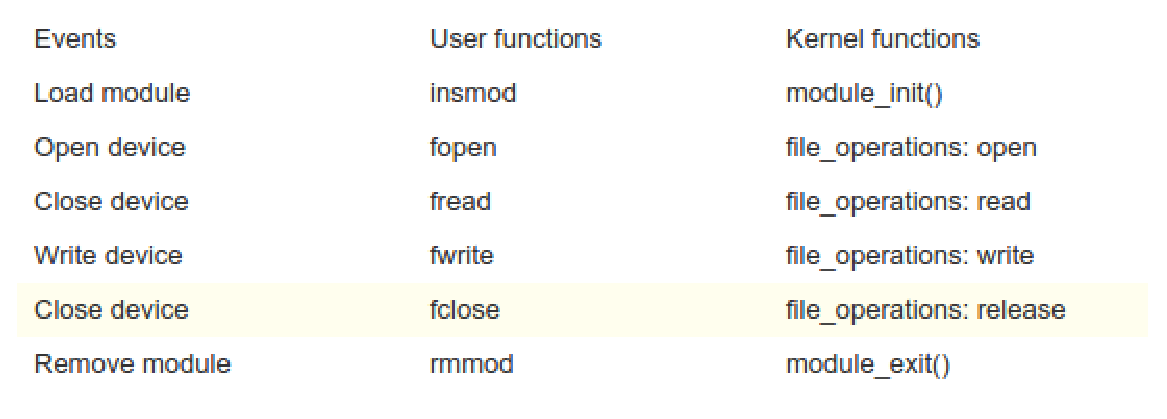
\includegraphics[width=0.9\textwidth]{figure/tabela.eps}
\end{figure}

Assim, por exemplo no espaço do usuário, para instalar o módulo é feita a chamada a função \textbf{insmod} passando
como argumento o módulo a ser carregado. Em seguida, no lado do kernel é chamada a função \textbf{module\_init()} de
modo que assim alguma tarefas , como reservar memória ram e portas de entrada e saída são executadas.
Por outro lado, para a remoçao de um módulo é feita a chamada de função \textbf{rmmod} passando como argumento
o módulo a ser removido, no lado do \textit{kernel} é chamada a função \textbf{module\_exit()}, liberando assim os recursos
de hardware alocados anteriormente. O codigo a seguir apresenta um \textit{hello word} tipico de \textit{device driver}.

\begin{figure}[H]
  \centering
  \caption{ Um \textit{Hello World} típico de \textit{device driver} }
  \label{fig:usblinux}
  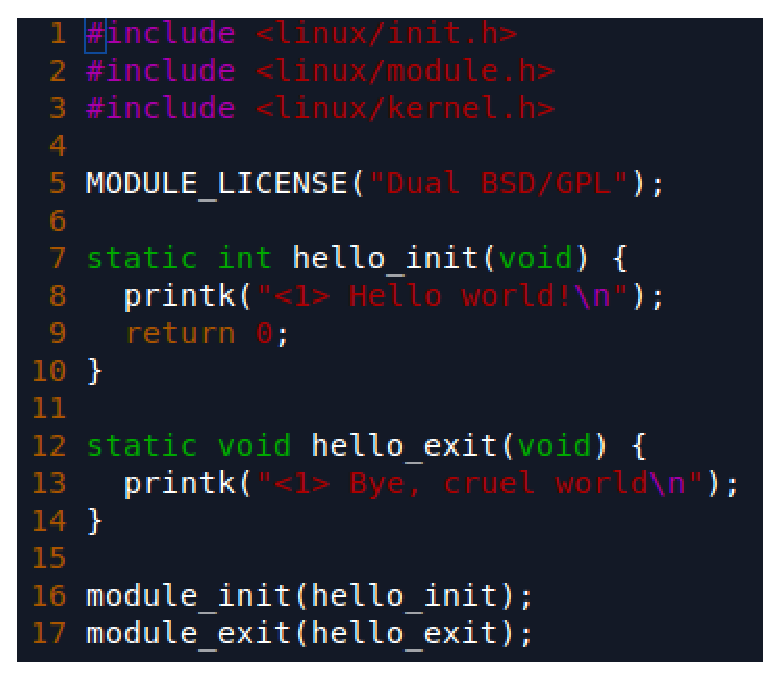
\includegraphics[width=0.5\textwidth]{figure/codigo.eps}
\end{figure}

Nas linhas de 1 a 3 são incluídas as bibliotecas utilizadas para uso de funções necessárias para 
construção de device drivers. Os métodos \textbf{hello\_init} e \textbf{hello\_exit} são executados quando um módulo 
é instalado e removido respectivamente. Destaca-se que esse métodos são passado para funções \textbf{ module\_init}
e \textbf{module\_exit} como argumento para que os mesmos sejam executados nessas operações ( instalação e 
remoção de módulos). Outro destaque é uso da função \textit{printk}, essa função possui ação semelhante a do \textit{printf}, 
entretanto ela típica do \textit{kernel} e imprime apenas nos arquivos de \textit{log} do sistema. Para compilação do código é
necessário o uso de Makefile com as seguintes linhas de código:

\begin{figure}[H]
  \centering
  \caption{ \textit{Makefile} utilizado para o programa \textit{hello.c} }
  \label{fig:usblinux}
  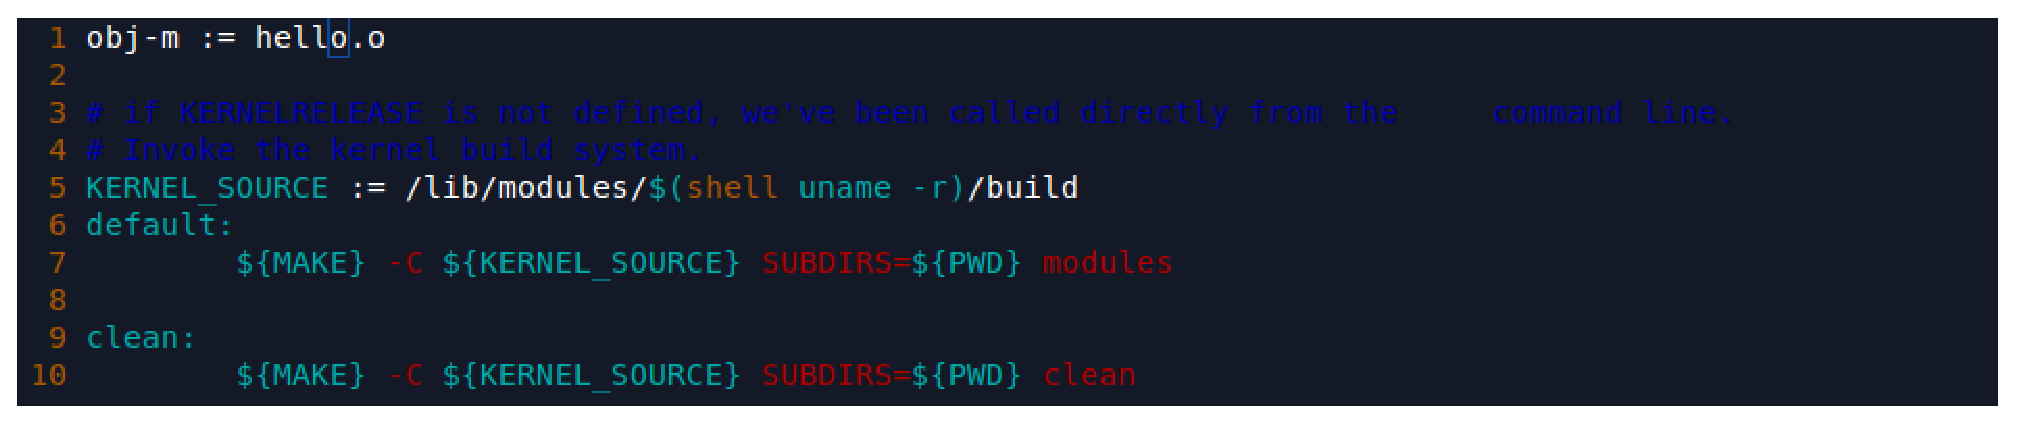
\includegraphics[width=0.9\textwidth]{figure/makefile.eps}
\end{figure}

\subsection{Vírus}

\begin{itemize}
  \item \textbf{Vírus de \textit{Boot}}: o vírus de boot foi um dos primeiros vírus a surgirem no mundo,
    ele foi criado com o objetivo de danificar o setor de inicialização do disco rígido,
    no qual a sua forma de propagação era através de um disquete contaminado. O vírus se
    alojava no primeiro setor do disco flexível e ocupava cerca de 1k ou menos em um
    disquete que era de 360k mais ou menos. Na inicialização do boot com o disquete
    contaminado, o vírus se aloja na memória no endereço 0000:7C00h da bios e começa
    a se auto-executar , prejudicando assim a inicialização do computador

  \item \textbf{Vírus de Macro}: o vírus macro encontrado-se frequentemente em documentos ou é
    inserido em códigos maliciosos em programas de processamento de texto, podendo ter
    origem em docs anexados ou em e-mails, no qual o vírus pode ser transferido para o
    computador depois de clicar em ligações de “phishing” ou mesmo em propagandas. Esses
    vírus são difíceis de serem identificados e o seu maior risco é que tem uma grande
    capacidade de se propagar, no qual eles podem causar danificações nos documentos infectados.
\end{itemize}

Maior parte dos vírus criados são desenvolvidos para a plataforma Windows, pois esse sistema operacional
é mais vulnerável porque ele não trabalha com múltiplos usuários nem com permissões de arquivos. Já a plataforma
Linux tem as definições bem claras sobre as permissões de arquivos, usuários e grupos, assim quando um SO Linux é
afetado por um vírus ele afetará somente o usuário que executou o programa, ao contrário do Windows, onde o que estiver
sendo executado acaba sendo afetado também pelos vírus. Assim, mesmo existindo vírus para o sistema operacional Linux, eles
só são propagados se forem executados por roots, assim eles não podem se espalhar remotamente, no qual afeta arquivos binários
na máquina ou disponíveis através de NFS.

%\lstinputlisting{virus.c}


%\end{lstlisting}

